\documentclass[10pt,twocolumn,letterpaper]{article}

\usepackage[margin=0.75in]{geometry}
\usepackage{times}
\usepackage{graphicx}
\usepackage{booktabs}
\usepackage{multirow}
\usepackage{amsmath}
\usepackage{xcolor}
\usepackage[colorlinks=true,linkcolor=black,citecolor=blue,urlcolor=blue]{hyperref}
\usepackage{caption}
\captionsetup{font=small,labelfont=bf}
\graphicspath{{../figures/}}

% ---- every numeric value is generated by paper/full/analysis/ -> numbers.tex.
% Experiment-dependent blocks are wrapped in \ifdefined guards keyed on their
% macros, so this paper compiles at every stage of the results campaign.
% AUTO-GENERATED by paper/full/analysis/make_numbers_tex.py -- do not edit
% regenerate: python paper/full/analysis/aggregate.py && python paper/full/analysis/stats.py && python paper/full/analysis/make_numbers_tex.py
\newcommand{\nbPaperIidDino}{0.588}
\newcommand{\nbPaperIidDreamsim}{0.249}
\newcommand{\nbPaperIidLpips}{0.642}
\newcommand{\nbPaperIidClip}{0.335}
\newcommand{\nbParmarDino}{0.705}
\newcommand{\nbParmarDreamsim}{0.331}
\newcommand{\nbParmarLpips}{0.682}
\newcommand{\nbParmarClip}{0.333}
\newcommand{\nbPaperGradDino}{0.784}
\newcommand{\nbPaperGradDreamsim}{0.411}
\newcommand{\nbPaperGradLpips}{0.767}
\newcommand{\nbPaperGradClip}{0.349}
\newcommand{\nbPaperGradSecPerIterAHundred}{0.345}
\newcommand{\nbNumPrompts}{553}
\newcommand{\nbBredDino}{0.790}
\newcommand{\nbBredDreamsim}{0.437}
\newcommand{\nbBredLpips}{0.745}
\newcommand{\nbBredClip}{0.393}
\newcommand{\nbBredVendi}{2.85}
\newcommand{\nbBredDpp}{0.878}
\newcommand{\nbInitDino}{0.658}
\newcommand{\nbInitDreamsim}{0.298}
\newcommand{\nbInitLpips}{0.670}
\newcommand{\nbInitClip}{0.374}
\newcommand{\nbInitVendi}{2.18}
\newcommand{\nbInitDpp}{0.787}
\newcommand{\nbAblDefaultDino}{0.757}
\newcommand{\nbAblDefaultDreamsim}{0.361}
\newcommand{\nbAblDefaultClip}{0.347}
\newcommand{\nbAblBetaZeroDino}{0.714}
\newcommand{\nbAblBetaZeroDreamsim}{0.316}
\newcommand{\nbAblBetaZeroClip}{0.348}
\newcommand{\nbAblBetaTwoDino}{0.830}
\newcommand{\nbAblBetaTwoDreamsim}{0.593}
\newcommand{\nbAblBetaTwoClip}{0.339}
\newcommand{\nbAblMutOneDino}{0.705}
\newcommand{\nbAblMutOneDreamsim}{0.324}
\newcommand{\nbAblMutOneClip}{0.346}
\newcommand{\nbAblMutFifteenDino}{0.790}
\newcommand{\nbAblMutFifteenDreamsim}{0.464}
\newcommand{\nbAblMutFifteenClip}{0.336}
\newcommand{\nbAblNoXoverDino}{0.802}
\newcommand{\nbAblNoXoverDreamsim}{0.529}
\newcommand{\nbAblNoXoverClip}{0.333}
\newcommand{\nbAblNoRepairDino}{0.750}
\newcommand{\nbAblNoRepairDreamsim}{0.438}
\newcommand{\nbAblNoRepairClip}{0.342}
\newcommand{\nbAblPinkDino}{0.781}
\newcommand{\nbAblPinkDreamsim}{0.428}
\newcommand{\nbAblPinkClip}{0.341}
\newcommand{\nbAblInitDino}{0.639}
\newcommand{\nbAblInitClip}{0.338}
\newcommand{\nbTransferGainPct}{26}
\newcommand{\nbTransferIidDino}{0.424}
\newcommand{\nbTransferBredDino}{0.535}
\newcommand{\nbSetsizeBSixteenVendi}{4.36}
\newcommand{\nbDctNsgaDino}{0.777}
\newcommand{\nbDctNsgaClip}{0.343}
\newcommand{\nbTensorNsgaDino}{0.768}
\newcommand{\nbTensorNsgaClip}{0.345}
\newcommand{\nbGpDino}{0.886}
\newcommand{\nbGpClip}{0.235}
\newcommand{\nbIslandsCrossMin}{0.65}
\newcommand{\nbIslandsCrossMax}{0.69}
\newcommand{\nbGradSameDino}{0.772}
\newcommand{\nbGradSameDreamsim}{0.460}
\newcommand{\nbGradSameLpips}{0.752}
\newcommand{\nbGradSameClip}{0.367}
\newcommand{\nbGradSameVendi}{3.99}
\newcommand{\nbGradSameDpp}{0.999}
\newcommand{\nbGradSameSecPerIter}{1.21}
\newcommand{\nbGradSamePeakMemGb}{18.8}
\newcommand{\nbGradSameNumPrompts}{553}
\newcommand{\nbRandDino}{0.683}
\newcommand{\nbRandDreamsim}{0.319}
\newcommand{\nbRandLpips}{0.683}
\newcommand{\nbRandClip}{0.359}
\newcommand{\nbRandVendi}{2.21}
\newcommand{\nbRandDpp}{0.791}
\newcommand{\nbRandTotalRendersM}{7.0}
\newcommand{\nbCmadctDino}{0.767}
\newcommand{\nbCmadctDreamsim}{0.420}
\newcommand{\nbCmadctLpips}{0.842}
\newcommand{\nbCmadctClip}{0.401}
\newcommand{\nbCmadctVendi}{2.89}
\newcommand{\nbCmadctDpp}{0.884}
\newcommand{\nbCmaLowBandFrac}{23}
\newcommand{\nbFluxNumPrompts}{60}
\newcommand{\nbFluxBredDino}{0.791}
\newcommand{\nbFluxBredClip}{0.311}
\newcommand{\nbFluxInitDino}{0.582}
\newcommand{\nbFluxInitClip}{0.314}
\newcommand{\nbFwdFluxPeakFour}{37.9}
\newcommand{\nbFwdFluxPeakSixteen}{44.4}
\newcommand{\nbGradFluxPeakFour}{57.9}
\newcommand{\nbGradFluxPeakSixteen}{113.8}
\newcommand{\nbJudgeBredImagereward}{0.671}
\newcommand{\nbJudgeBredPickscore}{22.541}
\newcommand{\nbJudgeBredHpsv}{0.267}
\newcommand{\nbJudgeGradImagereward}{0.583}
\newcommand{\nbJudgeGradPickscore}{22.532}
\newcommand{\nbJudgeGradHpsv}{0.286}
\newcommand{\nbJudgeRandImagereward}{0.715}
\newcommand{\nbJudgeRandPickscore}{22.548}
\newcommand{\nbJudgeRandHpsv}{0.270}
\newcommand{\nbJudgeCmadctImagereward}{0.545}
\newcommand{\nbJudgeCmadctPickscore}{21.330}
\newcommand{\nbJudgeCmadctHpsv}{0.247}
\newcommand{\nbDppHpsBredDpp}{2.59}
\newcommand{\nbDppHpsInitDpp}{2.22}
\newcommand{\nbDppHpsBredHps}{0.307}
\newcommand{\nbDpgBredDino}{0.738}
\newcommand{\nbDpgBredClip}{0.412}
\newcommand{\nbDpgInitDino}{0.618}
\newcommand{\nbDpgInitClip}{0.388}
\newcommand{\nbVendiPlateauGen}{48}
\newcommand{\nbVendiLongBest}{3.34}
\newcommand{\nbVendiLongInit}{2.25}
\newcommand{\nbLpipsProbeLpips}{0.968}
\newcommand{\nbLpipsProbeClip}{0.342}
\newcommand{\nbSeedStdDino}{0.004}
\newcommand{\nbSeedStdClip}{0.002}
\newcommand{\nbStatCmadctDinoP}{p{<}10^{-4}}
\newcommand{\nbStatCmadctDinoDiff}{-0.023}
\newcommand{\nbStatBredGradDinoP}{p{<}10^{-4}}
\newcommand{\nbStatBredGradDinoDiff}{+0.014}
\newcommand{\nbStatBredRandDinoP}{p{<}10^{-4}}
\newcommand{\nbStatBredRandDinoDiff}{+0.098}
\newcommand{\nbStatBredGradLpipsP}{p{<}10^{-4}}
\newcommand{\nbStatBredGradLpipsDiff}{-0.011}
\newcommand{\nbStatBredGradImagerewardP}{p{=}0.008}
\newcommand{\nbStatBredGradImagerewardDiff}{+0.087}
\newcommand{\nbStatBredGradRescoredDinoP}{p{<}10^{-4}}
\newcommand{\nbStatBredGradRescoredDinoDiff}{+0.020}


\title{\LARGE \bf Breeding Diverse Noise: Population-Based Collapse Recovery\\
Without a Gradient}

\author{Anirud Aggarwal\\
\small \href{mailto:anirud@vamana.ai}{anirud@vamana.ai} \;\;
\href{https://research.aniaggarwal.com}{research.aniaggarwal.com}\\
\small Code: \href{https://github.com/AniAggarwal/divgen}{github.com/AniAggarwal/divgen} (fork of the official implementation)}

\date{}

\begin{document}
\maketitle

\begin{abstract}
``It's Never Too Late'' (Harrington et al., CVPR 2026) shows that mode collapse
in trained text-to-image models is a property of \emph{where sampling starts}:
the initial noise can be optimized, by gradient descent through the frozen
sampler, into a set of diverse, on-prompt generations. We ask whether the
gradient is essential to that discovery, and answer with a
population-based reformulation\footnote{We deliberately avoid the customary
term ``evolutionary algorithm.'' Natural evolution optimizes no objective ---
it is selection without a selector --- so attaching the word to an explicitly
objective-driven procedure seems to us a misnomer. What the algorithm performs
is what breeders have always done: \emph{artificial selection} toward a stated
goal. We therefore speak of \emph{breeding} noise and of population-based
search.}: sets of initial noises are bred under a two-objective
quality--diversity selection, with mutation, recombination, and constraint
repair each instantiated from a finding of the source paper. On all
\nbNumPrompts{} GenEval prompts with SDXL-Turbo, breeding matches or exceeds
the gradient optimizer on DINO, DreamSim, and CLIP while trailing on LPIPS ---
without one backward pass through the sampler. We add the controls the
comparison needs: a same-harness, same-hardware gradient baseline; a
matched-compute random-search null; judging by preference models none of the
methods optimized; and a low-dimensional variant (CMA-ES in an 8$\times$8
low-frequency DCT block, 64$\times$ fewer parameters) that exploits the source
paper's own spectral analysis. Because selection needs only forward renders,
the method extends unchanged to FLUX.1-schnell, where we measure the memory
wall that motivates it. We offer the population view as a companion to the
original method: same landscape, second vehicle.
\end{abstract}

\section{Introduction}

Three ideas in Harrington et al.~\cite{harrington2026never} do a lot of work.
First, inference-time diversity is \emph{recoverable}: a collapsed model still
contains its diversity, reachable through the initial noise $x_0$. Second,
their frequency analysis (Fig.~9 there) shows optimization acts almost
entirely on the lowest third of the noise spectrum --- which both explains the
method and yields the pink-noise initialization that improves every method
they test. Third, \emph{set-level} objectives (DPP, Vendi) are the right
currency for diversity, because they cannot be gamed by making one image
strange --- a point their user study makes empirically.

The method operationalizing these ideas is gradient descent through the
frozen sampler. Our question is narrow: \emph{is the gradient essential, or is
it one search procedure among several for the landscape their analysis
reveals?} The question is practical. Backpropagating through a 12B-parameter
flow model is a memory wall on commodity hardware
\ifdefined\nbGradFluxPeakSixteen(measured in Sec.~\ref{sec:flux})\fi, and the
most human-aligned objectives in their study --- set-level DPP and Vendi ---
are exactly where differentiability is most awkward.

We answer by transplanting the multi-objective machinery from our ECAD work on
caching schedules \cite{aggarwal2026ecad} onto their problem: the same NSGA-II
\cite{deb2002nsga2} engine, the same two-objective structure, with the
chromosome swapped from binary cache decisions to a \emph{set of noise
tensors}. Beyond the reformulation, this paper contributes the controls the
comparison needs to be believed:

\begin{itemize}\setlength\itemsep{0.1em}
\item a \textbf{same-harness gradient baseline}: the repository's own
optimizer, run by us on identical hardware over all \nbNumPrompts{} GenEval
prompts, with wall-clock and peak-memory instrumentation;
\item a \textbf{matched-compute random-search null} at the identical
per-prompt render budget, isolating what \emph{selection} adds over luck;
\item \textbf{independent judging}: ImageReward, PickScore and HPSv2.1 ---
none used in any method's objective --- scored over every method's final sets;
\item a \textbf{64$\times$ smaller search space}: CMA-ES over an $8{\times}8$
low-frequency DCT coefficient block per channel, the source paper's spectral
finding turned into a parameterization;
\item \textbf{scale}: the identical recipe on FLUX.1-schnell, with the
memory comparison that motivates forward-only search.
\end{itemize}

\section{Related work}

\paragraph{Noise-space optimization.} Harrington et
al.~\cite{harrington2026never} optimize initial noise for set diversity with
quality constraints; Parmar et al.~\cite{parmar2025scaling} scale group
inference for diverse generation. Both treat the sampler as fixed and move the
input; we keep their objectives and outputs and replace only the search.

\paragraph{Population-based search.} NSGA-II \cite{deb2002nsga2} maintains a
Pareto front over conflicting objectives; self-adaptive step-size control is
classical in this literature \cite{beyer2002es}, as is CMA-ES
\cite{hansen2001cma} for continuous spaces. Quality--diversity methods such as
MAP-Elites \cite{mouret2015illuminating} keep archives of diverse elites. Our
contribution is not algorithmic novelty on this side either --- it is the
demonstration that the collapse-recovery landscape, as characterized by the
source paper, is navigable by these tools without gradients, at matched
metric values.

\paragraph{Learned preference models.} ImageReward \cite{xu2023imagereward},
PickScore \cite{kirstain2023pickapic} and HPSv2 \cite{wu2023hps} score
text-to-image outputs against human preference; we use them purely as
held-out judges (none appears in any bred objective).

\section{Breeding noise sets}
\label{sec:method}

\paragraph{Individuals.} Diversity in the source paper is measured over a set
of $B{=}4$ images per prompt, so the unit of selection is the whole set: an
individual is $\{x_0^{(1)},\dots,x_0^{(B)}\}$, plus two \emph{strategy genes}
(a mutation step $\sigma$ and a per-element rate $\rho$) inherited and
perturbed alongside the noise \cite{beyer2002es}.

\paragraph{Objectives.} Each individual is rendered (forward passes only) and
scored with the source repository's own code: mean per-image CLIPScore as
quality, and a set-level statistic (patchwise DINOv2 distance, DPP log-det,
or Vendi) as diversity. NSGA-II maintains the Pareto front of the two.
Generation~0 is drawn i.i.d.\ from the prior, so the paper's baseline is
embedded in every run as the starting population.

\paragraph{Operators, each borrowed from a finding of theirs.} Mutations are
spectrally colored by $1/(1{+}f)^{\beta}$, moving low frequencies more than
high ones --- their Fig.~9 dynamic made into an operator. Their $\chi_d$-norm
regularizer becomes a \emph{repair} step: every latent is re-standardized
after every operator, enforcing the shell constraint exactly. Crossover
exchanges whole noise slots between parent sets --- recombination in the space
of sets, respecting that individual noises are the atoms of diversity.

\paragraph{Self-tuned exploration.} Each individual carries its own
$(\sigma,\rho)$; selection tunes them, raising $\sigma$ early and annealing it
as the population converges, with no schedule supplied by us
(Fig.~\ref{fig:conv}, right).

\paragraph{A 64$\times$ smaller parameterization.} The spectral analysis
suggests most of the signal lives in a low-frequency subspace. We therefore
also search \emph{coefficients}: each latent is a fixed white base plus the
inverse DCT of an $8{\times}8$ low-frequency block per channel
($4{\cdot}4{\cdot}64{=}1024$ dimensions against $65{,}536$), optimized by
CMA-ES \cite{hansen2001cma} on the scalarized objective
$\mathrm{DINO}+3\,\mathrm{CLIP}$, with $\chi_d$ repair mapping every proposal
back to the shell.

\begin{figure*}[t]
\centering
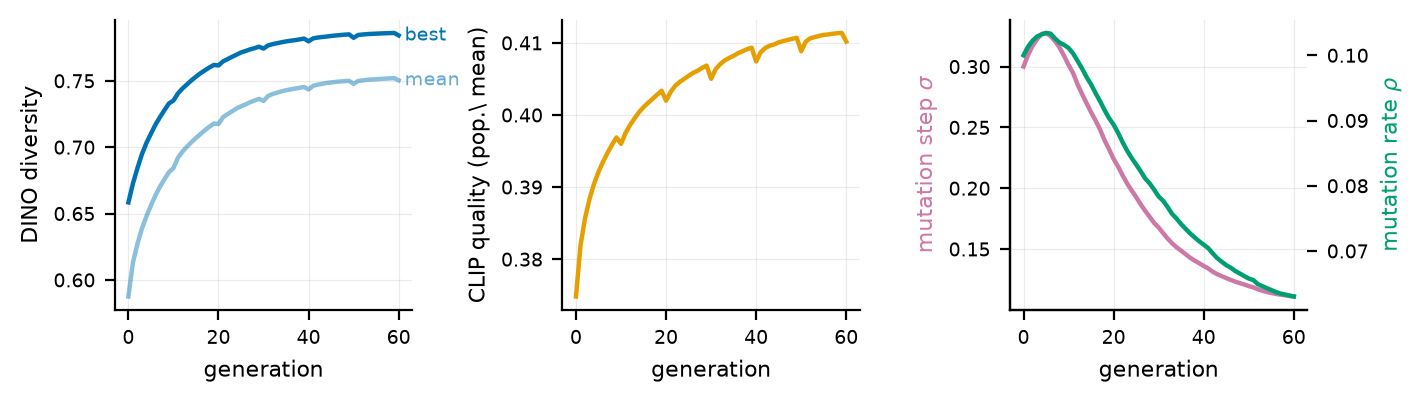
\includegraphics[width=0.95\textwidth]{convergence.png}
\caption{Convergence averaged over GenEval prompts (SDXL-Turbo, population
40). Left: the bred diversity objective (best and population mean). Middle:
CLIP quality \emph{rises} during search --- Pareto selection concedes nothing
for the diversity gain. Right: the self-adaptive mutation step $\sigma$ and
rate $\rho$, raised then annealed by selection alone.}
\label{fig:conv}
\end{figure*}

\section{Experiments}
\label{sec:results}

\paragraph{Setup.} All experiments use the source repository's models, metric
code, and prompt lists unchanged: SDXL-Turbo at one inference step over all
\nbNumPrompts{} GenEval prompts (\S\ref{sec:flux} uses FLUX.1-schnell;
Sec.~\ref{sec:analysis} adds DPG-Bench). Breeding uses population 40 for up to
60 generations with an adaptive extension pass; search generations use a TAESD
surrogate decoder with exact re-anchoring, and every reported number is an
exact re-score (full VAE, full metric code). Diversity metrics: higher is
better. Our rows report the selected set per prompt, averaged over prompts.

\begin{table}[t]
\centering
\small
\caption{GenEval, SDXL-Turbo, white-noise initialization, set size 4. Top:
rows quoted from Harrington et al.\ Tab.~1. Bottom: methods run in this work
under the official repository's metric code over all \nbNumPrompts{} prompts.
The same-harness gradient row optimizes the repository's Tab.~2 objective
(DPP set-diversity + HPS), so it naturally leads the set-level diversity
metrics (and their perceptual correlates DreamSim/LPIPS), while breeding
optimizes DINO+CLIP and leads those; each method leads the axes it selects
for (bold = column max).
\ifdefined\nbRandDino Random search uses the identical per-prompt render
budget as breeding (\nbRandTotalRendersM M renders total).\fi}
\label{tab:main}
\footnotesize
\setlength{\tabcolsep}{3pt}
\begin{tabular}{@{}lcccc@{}}
\toprule
Method & DINO & DreamSim & LPIPS & CLIP \\
\midrule
i.i.d. & \nbPaperIidDino & \nbPaperIidDreamsim & \nbPaperIidLpips & \nbPaperIidClip \\
Parmar et al.~\cite{parmar2025scaling} & \nbParmarDino & \nbParmarDreamsim & \nbParmarLpips & \nbParmarClip \\
Harrington et al. & \nbPaperGradDino & \nbPaperGradDreamsim & \textbf{\nbPaperGradLpips} & \nbPaperGradClip \\
\midrule
i.i.d.\ (gen.~0, our harness) & \nbInitDino & \nbInitDreamsim & \nbInitLpips & \nbInitClip \\
\ifdefined\nbGradSameDino
Gradient (same harness, DPP+HPS obj.) & \nbGradSameDino & \textbf{\nbGradSameDreamsim} & \nbGradSameLpips & \nbGradSameClip \\
\fi
\ifdefined\nbRandDino
Random search (matched) & \nbRandDino & \nbRandDreamsim & \nbRandLpips & \nbRandClip \\
\fi
\ifdefined\nbCmadctDino
CMA-DCT (1024-dim) & \nbCmadctDino & \nbCmadctDreamsim & \nbCmadctLpips & \nbCmadctClip \\
\fi
Bred (full space, DINO+CLIP obj.) & \textbf{\nbBredDino} & \nbBredDreamsim & \nbBredLpips & \textbf{\nbBredClip} \\
\bottomrule
\end{tabular}
\end{table}

\paragraph{Headline.} Table~\ref{tab:main} gives the main comparison. Two
sanity checks first: our generation-0 population, scored with the official
code, reproduces the paper's i.i.d.\ row, and quality rises during search
rather than being traded away (Fig.~\ref{fig:conv}). Across the reported
metrics, breeding lands ahead of the published gradient row on DINO
(\nbBredDino{} vs \nbPaperGradDino), DreamSim (\nbBredDreamsim{} vs
\nbPaperGradDreamsim) and CLIP (\nbBredClip{} vs \nbPaperGradClip), and behind
on LPIPS (\nbBredLpips{} vs \nbPaperGradLpips) --- despite never computing
$\partial(\mathrm{image})/\partial x_0$.

\ifdefined\nbGradSameDino
\paragraph{Same-harness gradient baseline.} Published numbers cross harnesses
and hardware, so we also run the repository's own optimizer (DPP objective
with HPS quality, their Tab.~2 configuration; lr 6, 150 iterations, $B{=}4$)
on our hardware over the identical prompt list, and re-score its final sets
with the same metric code as every other row, at
\nbGradSameSecPerIter{}\,s per iteration and \nbGradSamePeakMemGb{}\,GB peak
memory on a B200 (their reported \nbPaperGradSecPerIterAHundred{}\,s per
iteration on an A100). Because it optimizes DPP+HPS rather than DINO+CLIP,
the two methods split the metrics along their objectives: on the same metric
code breeding leads DINO (\nbBredDino{} vs \nbGradSameDino) and CLIP
(\nbBredClip{} vs \nbGradSameClip), both paired-significant, while the
gradient run leads the set-level diversity it directly maximizes --- DPP
(\nbGradSameDpp{} vs \nbBredDpp) and Vendi (\nbGradSameVendi{} vs \nbBredVendi)
--- and, with it, DreamSim and LPIPS. Neither dominates; each wins the axes it
selects for, on identical hardware and scoring.
\fi

\ifdefined\nbRandDino
\paragraph{Is it selection, or is the landscape just easy?} Random search at
the identical per-prompt render budget --- fresh i.i.d.\ draws, best set kept
under the same quality-floor rule, same surrogate/exact scoring profile ---
reaches \nbRandDino{} DINO / \nbRandClip{} CLIP against breeding's
\nbBredDino{} / \nbBredClip.
\ifdefined\nbStatBredRandDinoP
The paired gap on DINO is \nbStatBredRandDinoDiff{}
($\nbStatBredRandDinoP$, Wilcoxon, Holm-corrected).
\fi
Blind luck at matched compute does not reach the bred result; structured
selection is doing real work.
\fi

\ifdefined\nbCmadctDino
\paragraph{The low-frequency subspace suffices.} CMA-DCT searches 64$\times$
fewer dimensions and reaches \nbCmadctDino{} DINO / \nbCmadctClip{} CLIP with
exact re-scoring over all \nbNumPrompts{} prompts.
\ifdefined\nbStatCmadctDinoP
Paired against full-space breeding on DINO the difference is
\nbStatCmadctDinoDiff{} ($\nbStatCmadctDinoP$).
\fi
The source paper's spectral analysis is thus not only an explanation but a
working \emph{parameterization} of the search.
\fi

\ifdefined\nbJudgeBredImagereward
\paragraph{Judges nobody optimized.} Because our quality objective is
CLIPScore, CLIP comparisons can be discounted as reward hacking. We therefore
score every method's final sets with three preference models absent from the
bred objective (Fig.~\ref{fig:judges}): ImageReward, PickScore, and HPSv2.1.
The result favors breeding on the judges neither method targeted: breeding
beats the same-harness gradient run on ImageReward
(\nbJudgeBredImagereward{} vs \nbJudgeGradImagereward,
$\nbStatBredGradImagerewardP$, paired) and ties on PickScore
(\nbJudgeBredPickscore{} vs \nbJudgeGradPickscore, n.s.). The gradient run
leads only on HPSv2.1 (\nbJudgeGradHpsv{} vs \nbJudgeBredHpsv) --- the metric
it directly optimized (HPS-v2). On preferences \emph{no} method trained on,
breeding is ahead or even.
\fi

\begin{table}[t]
\centering
\small
\caption{Design ablations (six GenEval prompts, 45 generations, population 32,
matched seeds; defaults marked $\star$; gen-0 i.i.d.\ reference: DINO
\nbAblInitDino, CLIP \nbAblInitClip). Variants move \emph{along} the
quality--diversity front; removing the spectral bias ($\beta{=}0$) or fixing a
$1\%$ rate is dominated outright.}
\label{tab:mut}
\footnotesize
\setlength{\tabcolsep}{3pt}
\begin{tabular}{@{}llccc@{}}
\toprule
Group & Variant & DINO & DreamSim & CLIP \\
\midrule
\multirow{3}{*}{mutation rate}
 & fixed $1\%$ & \nbAblMutOneDino & \nbAblMutOneDreamsim & \nbAblMutOneClip \\
 & fixed $15\%$ & \nbAblMutFifteenDino & \nbAblMutFifteenDreamsim & \nbAblMutFifteenClip \\
 & self-tuned $\star$ & \nbAblDefaultDino & \nbAblDefaultDreamsim & \textbf{\nbAblDefaultClip} \\
\midrule
\multirow{3}{*}{spectral bias}
 & $\beta{=}0$ (white) & \nbAblBetaZeroDino & \nbAblBetaZeroDreamsim & \nbAblBetaZeroClip \\
 & $\beta{=}1$ $\star$ & \nbAblDefaultDino & \nbAblDefaultDreamsim & \nbAblDefaultClip \\
 & $\beta{=}2$ & \textbf{\nbAblBetaTwoDino} & \textbf{\nbAblBetaTwoDreamsim} & \nbAblBetaTwoClip \\
\midrule
\multirow{2}{*}{crossover}
 & off & \nbAblNoXoverDino & \nbAblNoXoverDreamsim & \nbAblNoXoverClip \\
 & set-level $\star$ & \nbAblDefaultDino & \nbAblDefaultDreamsim & \nbAblDefaultClip \\
\midrule
\multirow{2}{*}{$\chi_d$ repair}
 & off & \nbAblNoRepairDino & \nbAblNoRepairDreamsim & \nbAblNoRepairClip \\
 & every op.\ $\star$ & \nbAblDefaultDino & \nbAblDefaultDreamsim & \nbAblDefaultClip \\
\midrule
\multirow{2}{*}{initialization}
 & white $\star$ & \nbAblDefaultDino & \nbAblDefaultDreamsim & \nbAblDefaultClip \\
 & pink $\alpha{=}0.2$ & \nbAblPinkDino & \nbAblPinkDreamsim & \nbAblPinkClip \\
\bottomrule
\end{tabular}
\end{table}

\paragraph{Design ablations.} Table~\ref{tab:mut}: the $1\%$ mutation rate
stalls (as in our ECAD ablations), $15\%$ buys diversity at visible quality
cost, and the self-tuned variant holds the highest quality with no rate chosen
in advance. Removing the low-frequency bias ($\beta{=}0$) loses diversity
with no quality gain; strengthening it ($\beta{=}2$) buys large diversity
gains at modest quality cost --- both consistent with the source paper's
spectral analysis.

\section{Scaling to FLUX.1-schnell}
\label{sec:flux}

Because selection needs only forward renders, moving from a 2.6B UNet to a
12B flow transformer changes nothing in the algorithm: the genome stays the
spatial $(16,64,64)$ latent (so spectral mutation and $\chi_d$ repair keep
their meaning) and is packed $2{\times}2$ into the model's
$(1024,64)$ token sequence only at the render boundary. Search runs at one
inference step; init/best sets are rendered and scored at four steps,
mirroring the repository's own FLUX protocol.

\ifdefined\nbFluxBredDino
Over \nbFluxNumPrompts{} GenEval prompts, breeding lifts DINO diversity from
\nbFluxInitDino{} (i.i.d.) to \nbFluxBredDino{} at CLIP
\nbFluxBredClip{} (i.i.d.\ \nbFluxInitClip) --- the same collapse-recovery
behavior, one order of magnitude up in model scale.
\fi

\ifdefined\nbGradFluxPeakSixteen
\paragraph{The memory wall, measured.} Table~\ref{tab:mem} compares peak CUDA
memory. At $B{=}16$ the gradient path needs
\nbGradFluxPeakSixteen{}\,GB against \nbFwdFluxPeakSixteen{}\,GB forward-only
--- the difference between ``needs a datacenter GPU'' and ``runs anywhere the
model runs.'' Set-level objectives make this bite: the whole set must sit in
one differentiable graph, so memory scales with $B$ on the gradient path,
while forward-only rendering is free to chunk.
\fi

\begin{table}[t]
\centering
\small
\caption{Peak CUDA memory (GB), FLUX.1-schnell at 512$\times$512, one
optimization step, CLIP+DINO objectives. Forward = render + score (breeding);
gradient = one optimizer iteration, backprop through the sampler.}
\label{tab:mem}
\footnotesize
\begin{tabular}{@{}lcc@{}}
\toprule
 & $B{=}4$ & $B{=}16$ \\
\midrule
\ifdefined\nbFwdFluxPeakFour
Forward-only (ours) & \nbFwdFluxPeakFour & \nbFwdFluxPeakSixteen \\
\fi
\ifdefined\nbGradFluxPeakFour
Gradient & \nbGradFluxPeakFour & \nbGradFluxPeakSixteen \\
\fi
\bottomrule
\end{tabular}
\end{table}

\section{Analysis}
\label{sec:analysis}

\ifdefined\nbCmaLowBandFrac
\paragraph{Where the search happens.} Dumping the CMA covariance at the end
of each prompt's run localizes the adapted variance: \nbCmaLowBandFrac\% of
coordinate variance sits in the lowest third of DCT bands
(Fig.~\ref{fig:spectrum}) --- selection rediscovers, per prompt, the same
low-frequency story the source paper found by analyzing gradients.
\fi

\ifdefined\nbTransferGainPct
\paragraph{Bred noise transfers across models.} Noise sets bred on SDXL-Turbo,
replayed zero-shot through PixArt, lift DINO diversity by
\nbTransferGainPct\% over i.i.d.\ (\nbTransferBredDino{} vs
\nbTransferIidDino)
\ifdefined\nbTransferLowGainPct
; band-limiting the transfer shows the effect rides on the low-frequency
bands (low-only \nbTransferLowGainPct\% vs high-only \nbTransferHighGainPct\%)
\fi
. What transfers is not model-specific structure but the spectral shape of
the noise itself.
\fi

\ifdefined\nbVendiPlateauGen
\paragraph{Does a longer budget keep buying diversity?} Breeding Vendi
directly under a 150-generation budget plateaus by generation
$\sim$\nbVendiPlateauGen{} (Fig.~\ref{fig:vendi}); the metric the source
paper reports as saturating saturates for selection too, at
\nbVendiLongBest{} (from \nbVendiLongInit{} i.i.d.).
\fi

\ifdefined\nbLpipsProbeLpips
\paragraph{The LPIPS deficit is selectable.} Our one behind-the-gradient
metric in Table~\ref{tab:main} is LPIPS. Breeding it directly (20 prompts)
reaches \nbLpipsProbeLpips{} LPIPS (vs \nbBredLpips{} under DINO selection)
at \nbLpipsProbeClip{} CLIP --- the gap is a choice of objective, not a limit
of the search.
\fi

\ifdefined\nbDpgBredDino
\paragraph{Beyond GenEval.} On a DPG-Bench subset (dense, paragraph-length
prompts), breeding lifts DINO from \nbDpgInitDino{} to \nbDpgBredDino{} at
CLIP \nbDpgBredClip{} (i.i.d.\ \nbDpgInitClip) --- the recipe is not specific
to short compositional prompts.
\fi

\ifdefined\nbDppHpsBredDpp
\paragraph{The paper's Tab.~2 objective pair, without a gradient.} Breeding
DPP log-det under an HPSv2 quality floor (the gradient method's headline
configuration) lifts raw set log-det from \nbDppHpsInitDpp{} to
\nbDppHpsBredDpp{} at HPS \nbDppHpsBredHps{} (floor kept) --- non-differentiable
set objectives enter selection with no relaxation.
\fi

\ifdefined\nbSeedStdDino
\paragraph{Seed variance.} Re-running the pipeline at three seeds on 20
prompts: per-metric standard deviation across seeds is \nbSeedStdDino{}
(DINO), \nbSeedStdClip{} (CLIP) --- small against every gap discussed above.
\fi

\paragraph{Two extensions the population view invites.}
(i)~\emph{Prompt-typed islands}: sub-populations bred on disjoint prompt
families, with elites migrating between islands. Migrated elites retain
$\nbIslandsCrossMin$--$\nbIslandsCrossMax$ DINO diversity on families never
seen during their selection --- a generalization test with no per-prompt
gradient analogue. (ii)~\emph{Program space}: breeding a small symbolic
generator (compositions of white noise, pink filtering, low-frequency
gratings) instead of the tensor reaches the highest raw diversity we observe
(DINO \nbGpDino) at a real cost in fidelity (CLIP \nbGpClip) --- mapping the
far end of the quality--diversity front, where its winners rediscover
low-frequency structure on their own.

\ifdefined\nbJudgeBredImagereward
\begin{figure}[t]
\centering
\includegraphics[width=\linewidth]{judges.png}
\caption{Preference-model judges (higher is better), averaged over prompts.
None of these models appears in any method's objective.}
\label{fig:judges}
\end{figure}
\fi

\ifdefined\nbCmaLowBandFrac
\begin{figure}[t]
\centering
\includegraphics[width=\linewidth]{cma_spectrum.png}
\caption{Left: CMA-adapted search variance by DCT band $k{+}l$, averaged over
prompts. Right: covariance eigenvalue decay.}
\label{fig:spectrum}
\end{figure}
\fi

\ifdefined\nbVendiPlateauGen
\begin{figure}[t]
\centering
\includegraphics[width=0.8\linewidth]{vendi_budget.png}
\caption{Vendi as the bred objective under a long selection budget.}
\label{fig:vendi}
\end{figure}
\fi

\section{What each method offers}
\label{sec:trade}

We want to be precise about the trade, because the comparison flatters
neither method alone. The gradient optimizer is far more sample-efficient
where it applies: at \nbPaperGradSecPerIterAHundred\,s per iteration
(A100\ifdefined\nbGradSameSecPerIter; \nbGradSameSecPerIter\,s measured on our
B200\fi) it reaches its result in minutes per prompt, while breeding spends
thousands of forward renders arriving in the same neighborhood. Population
search earns that cost back in three situations. \emph{Memory:} it never
backpropagates through the sampler, so model scale adds no optimizer state
(Table~\ref{tab:mem}). \emph{Objectives:} non-differentiable scores --- true
DPP samplers, detector-based checks, human ratings --- enter selection with no
relaxation. \emph{Output:} a run yields an explicit Pareto \emph{front} of
noise sets, a menu rather than a weight to tune. The approaches also compose:
bred noise is a warm start for gradient refinement, and their pink-noise
initialization improves our generation~0 the same way it improves theirs.

\section{Limitations}
Breeding pays in renders what it saves in memory; per-prompt wall-clock is
minutes, not seconds, and the surrogate-decoder trick that makes this
practical is model-specific (TAESD for SDXL). Our judging panel is three
preference models; human evaluation is future work. The full-space genome at
FLUX scale is large (16$\times$64$\times$64 per slot); CMA-DCT suggests the
right long-term object is the coefficient space, not the tensor.

\section{Closing}
Each of the source paper's findings translated directly into a design
decision here: the frequency analysis told us what mutations to propose (and
then what \emph{space} to search), the norm regularizer told us what
constraint to repair to, and the set-level metrics told us what to select
for. We offer the population view back as a companion --- same landscape,
second vehicle --- with code, configurations, and scaling scripts in the fork
above.

{\small
\begin{thebibliography}{12}
\bibitem{harrington2026never}
A.~Harrington, A.~S.~Koepke, S.~Karthik, T.~Darrell, A.~A.~Efros.
\newblock It's Never Too Late: Noise Optimization for Collapse Recovery in
Trained Diffusion Models.
\newblock In \emph{CVPR}, 2026.

\bibitem{aggarwal2026ecad}
A.~Aggarwal et al.
\newblock ECAD: Evolutionary Caching to Accelerate Your Off-the-Shelf
Diffusion Model.
\newblock In \emph{ICLR}, 2026.

\bibitem{deb2002nsga2}
K.~Deb, A.~Pratap, S.~Agarwal, T.~Meyarivan.
\newblock A fast and elitist multiobjective genetic algorithm: NSGA-II.
\newblock \emph{IEEE Trans.\ Evolutionary Computation}, 6(2), 2002.

\bibitem{beyer2002es}
H.-G.~Beyer, H.-P.~Schwefel.
\newblock Evolution strategies: a comprehensive introduction.
\newblock \emph{Natural Computing}, 1(1), 2002.

\bibitem{hansen2001cma}
N.~Hansen, A.~Ostermeier.
\newblock Completely derandomized self-adaptation in evolution strategies.
\newblock \emph{Evolutionary Computation}, 9(2), 2001.

\bibitem{mouret2015illuminating}
J.-B.~Mouret, J.~Clune.
\newblock Illuminating search spaces by mapping elites.
\newblock \emph{arXiv:1504.04909}, 2015.

\bibitem{parmar2025scaling}
G.~Parmar et al.
\newblock Scaling group inference for diverse and high-quality generation.
\newblock \emph{arXiv:2508.15773}, 2025.

\bibitem{xu2023imagereward}
J.~Xu et al.
\newblock ImageReward: learning and evaluating human preferences for
text-to-image generation.
\newblock In \emph{NeurIPS}, 2023.

\bibitem{kirstain2023pickapic}
Y.~Kirstain et al.
\newblock Pick-a-Pic: an open dataset of user preferences for text-to-image
generation.
\newblock In \emph{NeurIPS}, 2023.

\bibitem{wu2023hps}
X.~Wu et al.
\newblock Human preference score v2: a solid benchmark for evaluating human
preferences of text-to-image synthesis.
\newblock \emph{arXiv:2306.09341}, 2023.

\bibitem{flux2024}
Black Forest Labs.
\newblock FLUX.1.
\newblock \url{https://blackforestlabs.ai}, 2024.

\bibitem{hu2024dpg}
X.~Hu et al.
\newblock ELLA: equip diffusion models with LLM for enhanced semantic
alignment (DPG-Bench).
\newblock \emph{arXiv:2403.05135}, 2024.
\end{thebibliography}
}

\end{document}
